\documentclass[12 pt]{article}

% Basic
\usepackage[utf8]{inputenc}
% \usepackage[spanish,mexico]{babel}

% Don't indent paragraphs, leave some space between them
\usepackage{parskip}
\usepackage{enumitem}
\usepackage{graphicx}
\usepackage{subfig}

% Math stuff
\usepackage{amsmath, amsfonts, mathtools, amsthm, amssymb}
\usepackage{breqn}
\usepackage{cancel}
\usepackage{etoolbox}
\usepackage{float}


% For neural networks
\usepackage{tikz}
\usetikzlibrary{matrix,chains,positioning,decorations.pathreplacing,arrows}

% Headers
\usepackage{fancyhdr}
\usepackage{lastpage}
\pagestyle{fancy}
\setlength{\headheight}{40pt}

% Commands
\newcommand\N{\ensuremath{\mathbb{N}}}
\newcommand\R{\ensuremath{\mathbb{R}}}
\newcommand\Z{\ensuremath{\mathbb{Z}}}
\newcommand\Q{\ensuremath{\mathbb{Q}}}
\newcommand\C{\ensuremath{\mathbb{C}}}

%Images
\usepackage{import}
\usepackage{xifthen}
\usepackage{pdfpages}
\usepackage{transparent}

\newcommand{\incfig}[1]{%
    \def\svgwidth{\columnwidth}
    \scalebox{.75}{\import{./figures/}{#1.pdf_tex}}
}

\newtheorem{teo}{Teorema}
\newtheorem{lema}{Lemma}

\newenvironment{solution}
  {\renewcommand\qedsymbol{$\blacksquare$}
  \begin{proof}[Proof]}
  {\end{proof}}
\renewcommand\qedsymbol{$\blacksquare$}


\begin{document}

\lhead{Deep Neural Networks}
\rhead{ Deep Learning specialization \\ Neural Networks and Deep Learning}
\cfoot{\thepage \ of \pageref{LastPage}}

\subsection*{Deep L-layer neural network}

In the former sessions we studied very shallow neural networks as the logistic regression
(one layer neural network) and a 2 layer Neural Network. In this session we will study
the more general case with $L$ layers neural networks. A three layer Neural Network
is shown below.

\begin{tikzpicture}[
    % define styles 
    clear/.style={ 
        draw=none,
        fill=none
    },
    net/.style={
        matrix of nodes,
        nodes={ draw, circle, inner sep=7 },
        nodes in empty cells,
        column sep=1cm,
        row sep=-9pt
    },
    >=latex
]
% define matrix mat to hold nodes
% using net as default style for cells
\matrix[net] (mat)
{
% Define layer headings
|[clear]| \parbox{1.3cm}{\centering Input\\layer} 
& |[clear]| \parbox{1.3cm}{\centering First Hidden\\layer} 
& |[clear]| \parbox{1.3cm}{\centering Second Hidden\\layer} 
& |[clear]| \parbox{1.3cm}{\centering Output\\layer} \\
|[clear]|  &              & |[clear]| & |[clear]| \\
$x_1$      & |[clear]|    &           & |[clear]|\\
|[clear]|  &              & |[clear]| & |[clear]| \\
$x_2$      & |[clear]|    &           &  \\
|[clear]|  &              & |[clear]| & |[clear]| \\
$x_3$      & |[clear]|    &           & |[clear]| \\
|[clear]|  &              & |[clear]| & |[clear]| \\
};

%lines from a_{i}^{0} to each a_{j}^{1}
\foreach \ai in {3,5,7} {
\foreach \aii in {2,4,6,8}
    \draw[->] (mat-\ai-1) -- (mat-\aii-2);
    }

\foreach \ai in {2,4,6,8} {
    \foreach \aii in {3,5,7}
        \draw[->] (mat-\ai-2) -- (mat-\aii-3);
        }

%lines from a_{i}^{1} to a_{0}^{2}
\foreach \ai in {3,5,7}
\draw[->] (mat-\ai-3) -- (mat-5-4);

% right most line with Output label
\draw[->] (mat-5-4) -- node[above] {$\hat{y}$} +(2cm,0);
\end{tikzpicture}

\textbf{Notation:}
\begin{align*}
    &L && \text{The number of layers in the neural network} \\
    &n^{[l]} && \text{The number of units in the layer } l \\
    &W^{[l]} && \text{The weights matrix in the layer } l \\
    &b^{[l]} && \text{The bias vector in the layer } l \\ \\
    &a^{[l]} && \text{Activation vector in the layer } l \\
    &a^{[0]} := x \\
    &a^{[l]} := \hat{y}
\end{align*}

\subsection*{Forward Propagation in a Deep Network}

For a the input $X = \begin{bmatrix} x^{(1)} | \cdots | x^{(m)} \end{bmatrix}$ 
the forward propagation is given by the following equations:
\begin{align*}
    Z^{[i]} &= W^{[i]}A^{[i-1]} + b^{[i]}  &&\forall i \in\{1,\dots,l\} \\
    A^{[i]} &= g^{[i]}(Z^{[i]}) && \forall i \in\{1,\dots,l\}
\end{align*}

It's extremely important (and sometimes really difficult) to get the right matrix 
dimensions
\begin{align*}
    W^{[i]} &\in \mathbb{R}^{n^{[i]} \times n^{[i-1]}} &&
    A^{[i]} \in \mathbb{R}^{n^{[i-1]} \times m} \\
    b^{[i]} &\in \mathbb{R}^{n^{[i]} \times m} &&
    Z^{[i]} \in \mathbb{R}^{n^{[i]} \times m} 
\end{align*}
\subsection*{Deep representations}
Why is it important for the neural networks to be \textit{deep} and have a lot of hidden
layers?

Intuitively, you can think of the earlier layers of the neural network as detecting 
simple functions. And then composing them together in the later 
layers of a neural network so that it can learn more and more complex functions.

This simple to complex hierarchical representation, or compositional representation, 
applies in several types of data loke images (for problems offace recognition) and 
audio (for problems of speech recognition)

The advantage of multiple layers is that they can learn features at various levels of 
abstraction. For example, if you train a deep convolutional neural network to classify 
images, you will find that the first layer will train itself to recognize very basic 
things like edges, the next layer will train itself to recognize collections of edges 
such as shapes, the next layer will train itself to recognize collections of shapes like 
eyes or noses, and the next layer will learn even higher-order features like faces. 
Multiple layers are much better at generalizing because they learn all the intermediate 
features between the raw data and the high-level classification.
\newpage
\subsection*{Forward and Backward Propagation}

When doing backward propagation for the layer $l$ we have
\begin{align*}
    &\text{Input: } \ \quad \quad da^{[l]} \\
    &\text{Output:} \quad \quad da^{[l-1]}, dW^{[l]}, db^{[l]}
\end{align*}
Where the gradients are given by:
\begin{align*}
    dZ^{[l]} &= dA^{[l]} * g^{[l]'} (Z^{[l]}) \\
    dW^{[l]} &= \frac{1}{m} dZ^{[l]} A^{[l-1]\top} \\
    db^{[l]} &= \frac{1}{n} sum(dZ^{[l]}) \\ 
    dA^{[l-1]} &= W^{[l]\top} dZ^{[l]}
\end{align*}

A summary of the forward and backward propagation process for a three layer neural 
network is ilustrated in the following image:

\begin{figure}[H]
    \begin{center}
            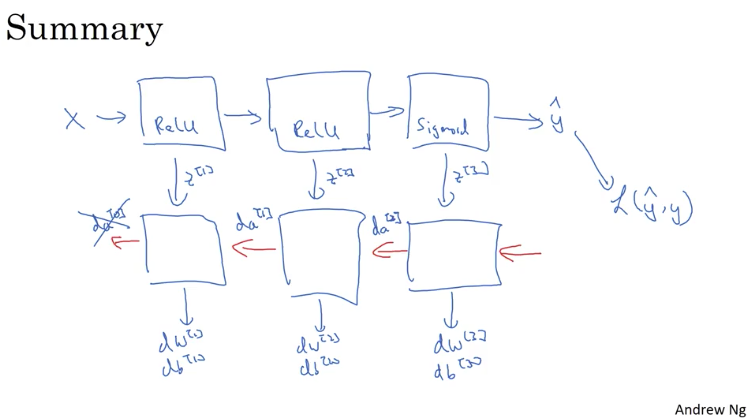
\includegraphics[width=0.9\textwidth]{img/summary.jpg}
        \end{center}
\end{figure}

\subsection*{Parameters vs hyperparameters}

Parameters:
\begin{align*}
    W^{[i]} \ \forall i \in \{1,...,L\} && \text{The weights matrix in each layer} \\
    b^{[i]} \ \forall i \in \{1,...,L\} && \text{The bias vector in each layer} 
\end{align*}

Hyperparameters:
\begin{align*}
    \alpha && \text{The learning rate} \\
    n_{iter} && \text{The number of iterations} \\
    L && \text{The number of hidden layers} \\
    n^{[i]} \ \forall i \in \{1,...,L\} && \text{The number of hidden units in each layer} \\
    n^{[i]} \ \forall i \in \{1,...,L\} && \text{The activation function for each layer}
\end{align*}

And several other hyperparameters like momentum, minibatch size and regularization.


\end{document}